The problem of determining similarity between data objects is a well-known and exhaustively researched area within computer vision and machine learning. 
A significant amount of the work for these tasks revolve around deep neural network architectures and large amounts of data - and are as such computationally expensive, and not well suited for experimentation with limited resources.
This project set out to examine low-cost methodologies for obtaining useful results. 
This section proposes a combination of techniques (supported by the literature) that may allow for fast, inexpensive training of models intended to perform reasonably well on image similarity tasks - not only for this particular domain, but perhaps many others.
Literature of particular interest for this project are; autoencoders and transfer learning and will be discussed below.

\subsection{Autoencoders as Feature Extractors}
Several works have addressed the capabilities of autoencoders as feature extraction models. 
Using autoencoders for feature extraction relies on the autoencoders ability to produce a low-dimensional representation of high-dimensional data within its bottleneck layer.
\newline
In \autocite{HintonScience2006}, \textbf{Hinton and Salakhutdinov} show that autoencoders can be trained to learn the most representative features in the bottleneck layer, allowing a decoder layer to reconstruct images from the Olivetti Face Dataset.
In the article, they achieve good reconstruction and feature extraction results employing a 30-dimensional autoencoder architecture. 
They show that this methodology generalizes well to also other domains. Additionally find that a deeper, 2000-500-250-125-2 autoencoder learns to construct representations that has a well-separated feature space for different classes of documents.
\newline
Autoencoders often learn data-specific features, and may in some scenarios not generalize well to new input - even in the same domain. 
\textbf{Vincent et al.}\autocite{Vincent2008} outline an approach for increasing robustness of autoencoder architectures by introducing the concept of Denoising Autoencoders.
This technique relies on corrupting input data prior to training such that the autoencoder learns useful internal representation by effectively reconstructing the corrupted input to its original state. 
They conclude by experimentation that corrupting the input to autoencoders is advantageous across several benchmarks. 
\newline
Supporting the idea that autoencoders are well suited as feature extractors, \textbf{Krizhevsky and Hinton}\autocite{Krizhevsky2010} propose the use of deep autoencoders for image retrieval. 
They exploit the autoencoders bottleneck layer to map images to much more compact binary representations to aid in searching for images in databases. 
Their work is based on a dataset consisting of 80 million tiny images and propose that deep autoencoders are capable of extracting more semantic information than other techniques.
Furthermore, they claim that this methodology allows for construction of better image hashes; allowing for faster, scalable image retrieval.
\newline
Going further, \textbf{Pulgar et al.}\autocite{Pulgar2018} propose a classifier based on autoencoders and \texttt{kNN} clustering. 
Here, they employ an autoencoder to reduce data dimensionality allowing the \texttt{kNN}-classifier to achieve significantly better classification results. 
This is possible due to the distance vectors calculated by the \texttt{kNN} are better separated due to the more information-dense, lower-dimensional encodings produced by the encoder.


\subsection{Training Strategies for Autoencoders} \label{sec:trainae}
Until quite recently, the training strategy of choice for autoencoders was greedy layer-wise pre-training. 
\textbf{Zhou et al.}\autocite{Zhou2014} argue that this approach has severe drawbacks in the form of suboptimal performance due to a discrepancy in learning of higher and lower layers of deeper models.
In this article, they show that joint training provides better learning of the data distribution model in autoencoders. 
It is suggested that this may hold for both supervised and unsupervised training scenarios with autoencoders. 
Furthermore, they find that employing regularization in the joint training scheme is crucial to model performance. 
Zhou et al. concluded that joint learning methods “...learn better data models, but also more representative features for classification as compared to the layer-wise method”.



\subsection{Transfer Learning Strategies}
Many machine learning methods have shown to work well under the assumption that training and test data are drawn from the same distribution. 
In cases where that distribution is subject to change - e.g. new data that is dissimilar to the original data on which the model was trained, machine learning models are not capable of adapting.
Thus, it is often the case, that models need to be retrained and/or reformulated to fit the new data - which is often impractical, expensive or even impossible. 
Furthermore, training a new model requires that new data is plentiful enough for the model to learn robust features related to this new underlying distribution. 
The idea behind transfer learning is to transfer features learned by one model into another.
\newline
\textbf{Pan and Yang}\autocite{PanYang2010} describe different forms of transfer learning in their survey article. 
They introduce the notion of inductive and transductive transfer learning settings - and elaborate on how to categorize transfer learning strategies for varying settings. 
In particular, \texttt{Domain Adaptation} is relevant to the work conducted in this project. 
In the article, Pan and Yang compares the performance of transfer-learned models - their results suggest, that it is often the case, that transfer learning can improve performance compared to other training strategies. 
Furthermore, their work suggest that transfer learning allow models to be trained in settings that would otherwise have been infeasible. 
\newline
The transferability of features is determined by what a model learns. 
Work by \textbf{Yosinski et al.}\autocite{Yosinski2014} and \textbf{Razavian et al.}\autocite{Razavian2014} suggest that deep neural networks learn generalizable features in the lower layers.
Generic descriptors obtained from deep neural networks' lower layers appear to learn features that are akin to Sobel, Gabor and color blob filters - which are used across a multitude of computer vision related settings.
This suggests, that the computational expenditures related to training a model for a new domain can be somewhat alleviated by exploiting features from other pretrained networks. 

\subsection{A modelling strategy}
Given the theory established so far, and the insights from previous scholars, a feature transfer from a pretrained network to an autoencoder architecture could yield robust results - and significantly decrease the training time.
Below, an outline of the modelling strategy is established.
Pass image data through a pretrained network; extract from a feature layer (before the final classification layer).
Train an autoencoder to replicate the feature layer. 
Extract encodings at the bottleneck layer of the autoencoder; obtain the cosine distance matrix and construct a prediction from the cosine distance matrix by finding the index with the largest similarity coefficient to the source data.

\begin{figure}[H]
    \centering
    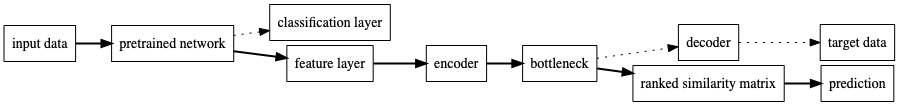
\includegraphics[scale=0.35]{pictures/graphviz/project}
    \caption{Outline of modeling strategy}
    \label{fig:strategy}
\end{figure}


